\documentclass{article}

\usepackage{amsmath, amsfonts, amsthm, amssymb} 
\usepackage{listings}
\usepackage{graphicx}
\usepackage{float}
\usepackage{subfigure}
\usepackage{geometry}
\usepackage{hyperref}
\usepackage[parfill]{parskip} % no newline indent
\usepackage{enumitem} % enumerate / ordered list
\usepackage{booktabs} % three-line table
\usepackage{array}   % for \newcolumntype macro
\newcolumntype{C}{>{$}c<{$}} % math-mode version of "l" column type

\theoremstyle{definition} % difinition
\newtheorem{definition}{Definition}[section]
\newtheorem{theorem}{Theorem}[section]
\newtheorem{remark}{Remark}[section]

\newcommand{\dd}{\mathrm{d}}
\newcommand{\RR}{\mathbb{R}}
\newcommand{\NN}{\mathbb{N}}
\newcommand{\ZZ}{\mathbb{Z}}
\newcommand{\CC}{\mathbb{C}}
\newcommand{\PP}{\mathbb{P}}


\geometry{
	paper=a4paper, 
	top=2.5cm,
	bottom=2.5cm, 
	left=2.5cm, 
	right=3cm,
	headsep=0.75cm, 
}
\title{ROB 501 HW5}
\author{Yulun Zhuang \\ \href{mailto:yulunz@umich.edu}{yulunz@umich.edu}}
\date{\today}

\begin{document}

\maketitle

\section{}

\subsection{}

\begin{align*}
	A_3 &= 
	\begin{bmatrix}
		3 & 10 & 0\\
		0 & 2 & 4\\
		0 & 0 & 1
	\end{bmatrix}
	\\
	A_3 - \lambda I &= 
	\begin{bmatrix}
		3 - \lambda & 10 & 0\\
		0 & 2 - \lambda & 4\\
		0 & 0 & 1 - \lambda
	\end{bmatrix}
\end{align*}

Characteristic polynomial of $A_3$ is $det(A_3 - \lambda I)=(3-\lambda)(2-\lambda)(1-\lambda)$.
$$det(A_3 - \lambda I)=0 \Rightarrow \lambda = 1, 2, 3$$

When $\lambda=3$,
$
(A_3 - \lambda I)x_1 = \mathbf 0 \Rightarrow x_1 = [1, 0, 0]^T
$

When $\lambda=2$,
$
(A_3 - \lambda I)x_2 = \mathbf 0 \Rightarrow x_2 = [-10, 1, 0]^T
$

When $\lambda=1$,
$
(A_3 - \lambda I)x_3 = \mathbf 0 \Rightarrow x_3 = [20, -4, 1]^T
$


Let $\alpha_1 x_1 + \alpha_2 x_2 + \alpha_3 x_3 = 0$,

\begin{align*}
	&\underbrace{
		\begin{bmatrix}
			1 & -10 & 20\\
			0 & 1 & -4\\
			0 & 0 & 1
		\end{bmatrix}
	}_A
	\begin{bmatrix}
		\alpha_1 \\ \alpha_2 \\ \alpha_3
	\end{bmatrix}
	= 0 
	\\
	\Rightarrow &\ det(A) = 1 > 0\\
	\Rightarrow &\ \alpha_1 = \alpha_2 = \alpha_3 = 0
\end{align*}

The e-vectors of $A$ are linear independent.

\subsection{}

\begin{align*}
	A_4 &= 
	\begin{bmatrix}
		5 & 1 & 1\\
		0 & 5 & 3\\
		0 & 0 & 2
	\end{bmatrix}
\end{align*}

The e-values: $\lambda = 5, 5, 2$.

When $\lambda=5$,
$
(A_4 - \lambda I)x_1 = \mathbf 0 \Rightarrow x_1 = [1, 0, 0]^T
$

When $\lambda=2$,
$
(A_4 - \lambda I)x_2 = \mathbf 0 \Rightarrow x_2 = [0, -1, 1]^T
$

No, since $span\{x_1, x_2\} \neq \RR^3$. E.g. $v = [0, 0, 1]$ can not be represented by any combination of $x_1$ and $x_2$.

\section{}
Given $ B = P^{-1}AP$, show that $det(A-\lambda I) = det(B-\lambda I)$.

\begin{proof}
	\begin{align*}
		&det(B - \lambda I)\\
		=&\ det(P^{-1}AP - \lambda I)\\
		=&\ det(P^{-1}AP - P^{-1} \lambda I P)\\
		=&\ det(\left[P^{-1}(A - \lambda I) P\right])\\
		=&\ det(P^{-1})det(A - \lambda I)det(P)\\
		=&\ det(A - \lambda I)
	\end{align*}
\end{proof}

\section{}
Given $A_3$, whose e-values are $\lambda = 3, 2, 1$ and cooresponding e-vectors are $[1, 0, 0]^T,\ [-10, 1, 0]^T,\ [20, -4, 1]^T$, show that $A$ is similar to a diagonal matrix.

\begin{proof}
	\begin{align*}
		A_3 [x_1 \mid x_2 \mid x_3] &= [\lambda_1 x_1 \mid \lambda_2 x_2 \mid \lambda_3 x_3]\\
		&= 
		\underbrace{[x_1 \mid x_2 \mid x_3]}_P
		\underbrace{\begin{bmatrix}
			\lambda_1 & & \\
			& \lambda_2 & \\
			& & \lambda_3
		\end{bmatrix}
		}_\Lambda\\
		\Rightarrow A_3 = P\Lambda P^{-1}
	\end{align*}
\end{proof}

\section{}

\subsection{}
\begin{figure}[H]
    \centering
        \textsf{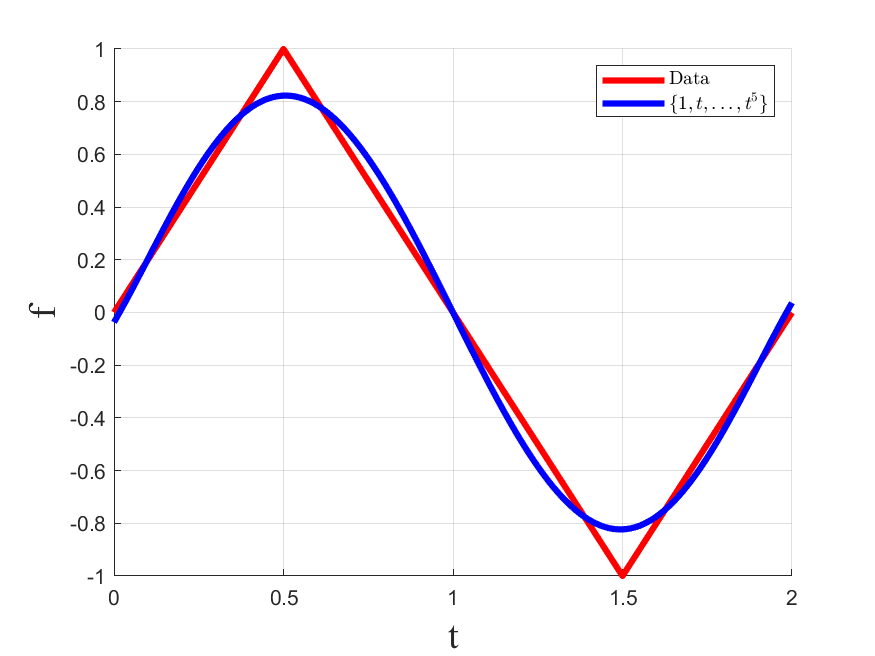
\includegraphics[width=0.6\columnwidth]{hw5-prob4-fig1.png}}
        \caption{Least square fit of the data using $\{1, t, \dots, t^5\}$}
        \label{fig: 4-1}
\end{figure}

Coefficients: $\boldsymbol \alpha =[
-0.0370,
 2.2158,
 2.8901,
-11.2271,
 7.6978,
-1.5396]^T.
$

\subsection{}
\begin{figure}[H]
    \centering
        \textsf{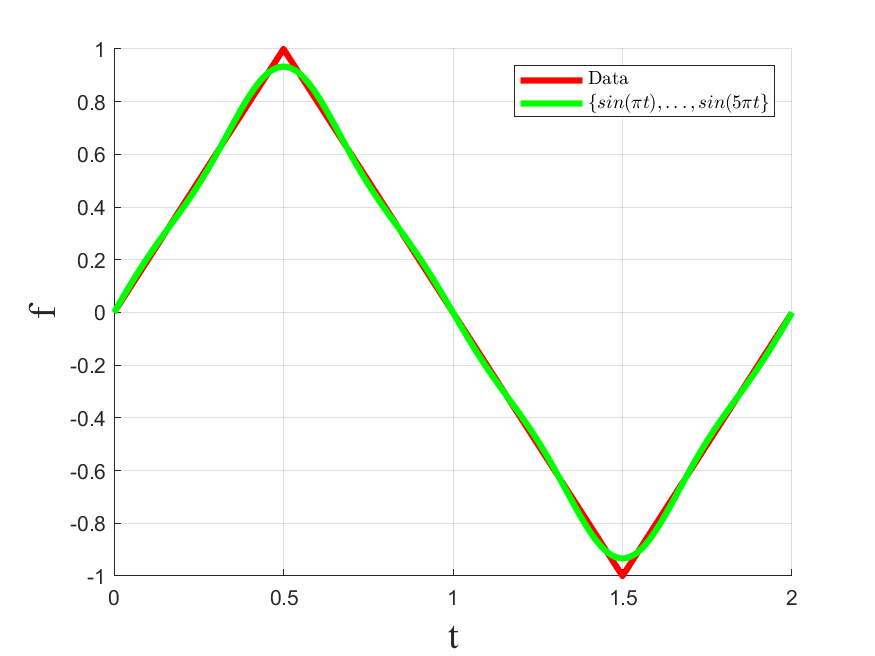
\includegraphics[width=0.6\columnwidth]{hw5-prob4-fig2.png}}
        \caption{Least square fit of the data using $\{sin(\pi t), \dots, sin(5\pi t)\}$}
        \label{fig: 4-2}
\end{figure}

Coefficients: $\boldsymbol \alpha =[
    0.8106,
    0.0000,
   -0.0901,
    0.0000,
    0.0325]^T.
$

\section{}

Function: $f(t) = \alpha_0 + \alpha_1 t + \alpha_2 t^2 + \alpha_3 t^3$

\begin{align*}
	&f'(t) = \frac{df(t)}{dt} = 3\alpha_3 t^2 + 2 \alpha_2 t + \alpha_1\\
	&f'(0.3) = -0.4016	
\end{align*}

\begin{figure}[H]
    \centering
        \textsf{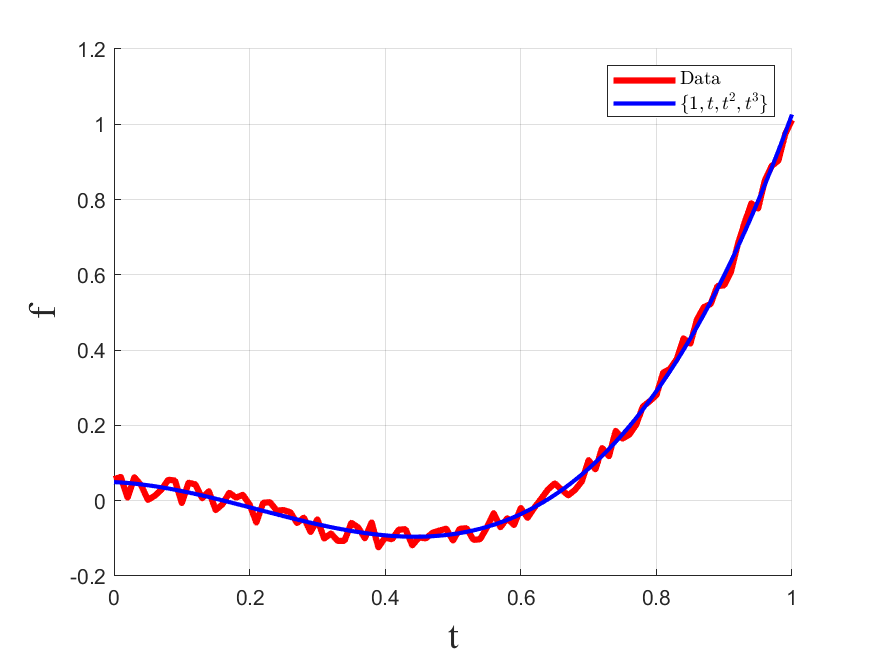
\includegraphics[width=0.6\columnwidth]{hw5-prob5-fig1.png}}
        \caption{Least square fit of the data using $\{1, t, t^2, t^3\}$}
        \label{fig: 5-1}
\end{figure}

Coefficients: $\boldsymbol \alpha =[
    0.0495,
   -0.0847,
   -1.8287,
    2.8900]^T.
$

\section{}
Show that on $(\CC^n, \CC)$, $<x, y> = x^T\bar{y}$ satisfies the difinition of inner product used in lecture, while $<x, y> = \bar{x}^T y$ satisfies the difinition of inner product in Nagy's book.

For part I, 

\begin{enumerate}[label=(\alph*)]
	\item \textbf{Hermitian Symmetry}: $\forall x, y\in \CC^n, \overline{<y, x>} = \overline{y^T\bar{x}} = \overline{\Sigma_{i=1}^ny_i\bar x_i} = \Sigma_{i=1}^nx_i\bar y_i = x^T\bar{y} = <x, y>$
	\item \textbf{Non-negativity}: $\forall x\in \CC^n, <x,x> = x^T\bar{x} = \Sigma_{i=1}^nx_i\bar{x_i} \ge 0$; when $<x,x>=0, |x_i|^2 = 0 \Rightarrow x=\mathbf 0$
	\item \textbf{Linearity in the first argument}:
	\begin{align*}
		\forall \alpha_1, \alpha_2& \in \CC, x_1, x_2, y \in \CC^n,\\
		&<\alpha_1 x_1 + \alpha_2 x_2,\ y> = (\alpha_1 x_1 + \alpha_2 x_2)^T\bar{y} = {\alpha_1 x_1}^T\bar{y} + {\alpha_2 x_2}^T\bar{y} = \alpha_1 <x_1, y> + \alpha_2 <x_2, y>
	\end{align*}
\end{enumerate}

For part II, 

\begin{enumerate}[label=(\alph*)]
	\item \textbf{Hermitian Symmetry}: $\forall x, y\in \CC^n, \overline{<y, x>} = \overline{\bar{y}^Tx} = \overline{\Sigma_{i=1}^n\bar y_ix_i} = \Sigma_{i=1}^n\bar x_iy_i = \bar{x}^Ty = <x, y>$
	\item \textbf{Non-negativity}: $\forall x\in \CC^n, <x,x> = \bar{x}^Tx = \Sigma_{i=1}^n\bar{x_i}x_i \ge 0$; when $<x,x>=0, |x_i|^2 = 0 \Rightarrow x=\mathbf 0$
	\item \textbf{Linearity in the second argument}:
	\begin{align*}
		\forall \alpha_1, \alpha_2& \in \CC, x, y_1, y_2 \in \CC^n,\\
		&<x,\ \alpha_1 y_1 + \alpha_2 y_2> = \bar{x}^T(\alpha_1 y_1 + \alpha_2 y_2) = \alpha_1 \bar{x}^T{y_1} + \alpha_2 \bar{x}^T{y_2} = \alpha_1 <x, y_1> + \alpha_2 <x, y_2>
	\end{align*}
\end{enumerate}

\section{}
Define the inner product $<p, q> = \int_{-1}^1 p(x)q(x)dx$ in $\PP_3([-1,1])$.

Show that the set $P = \{p_0, p_1, p_2, p_3\}$ is an orthogonal basis in $\PP_3$.


\begin{proof}

\begin{enumerate}[label=(\alph*)]
	\item $P$ is linear independent
	Let $\alpha_0 p_0 + \alpha_1 p_1 + \alpha_2 p_2 + \alpha_3 p_3 = 0$,
	
	\begin{align*}
		\frac{5}{2}\alpha_3 x^3 + \frac{3}{2}\alpha_2 x^2 + (\alpha_1 - \frac{3}{2}\alpha_3) x + (\alpha_0 - \frac{1}{2}\alpha_2) = 0\\
		\left\{
			\begin{array}{llll}
				\alpha_3 = 0\\
				\alpha_2 = 0\\
				\alpha_1 - \frac{3}{2}\alpha_3 = 0\\
				\alpha_0 - \frac{1}{2}\alpha_2 = 0
			\end{array}
		\right. 
		\Rightarrow
		\alpha_0 = \alpha_1 = \alpha_2 = \alpha_3 = 0
	\end{align*}
	
	\item $span\{p_0, \dots, p_3\} = \PP_3$
	$\forall x\in \PP_3, x=\beta_3 x^3 + \beta_2 x^2 + \beta_1 x + \beta_0$, we show that $x$ can be represented by $P$.
	
	\begin{align*}
		\left\{
			\begin{array}{llll}
				\frac{5}{2}\alpha_3 = \beta_3\\
				\frac{3}{2}\alpha_2 = \beta_2\\
				\alpha_1 - \frac{3}{2}\alpha_3 = \beta_1\\
				\alpha_0 - \frac{1}{2}\alpha_2 = \beta_0
			\end{array}
		\right. 
		\Rightarrow
		\left\{
			\begin{array}{llll}
				\alpha_0 = \beta_0 + \frac{1}{3}\beta_2\\
				\alpha_1 = \beta_1 + \frac{3}{5}\beta_3\\
				\alpha_2 = \frac{2}{3}\beta_2\\
				\alpha_3 = \frac{2}{5}\beta_0
			\end{array}
		\right. 
	\end{align*}
	
	\item The inner product of between elements in $P$ equal to 0.

	\begin{align*}
		&\left\langle p_0, p_3\right\rangle=\int_{-1}^1 \frac{1}{2}\left(5 x^3-3 x\right) d x=\int_{-1}^1\left(\frac{5}{2} x^3-\frac{3}{2}x \right)d x=\left.\left(\frac{5}{8} x^4-\frac{3}{4} x^2\right)\right|_{-1}^1=0 \\
		&\left\langle p_1, p_2\right\rangle=\int_{-1}^1 \frac{1}{2} x\left(3 x^2-1\right) d x=\int_{-1}^1\left(\frac{3}{2} x^3-\frac{1}{2} x\right) d x=\left.\left(\frac{3}{8} x^4-\frac{1}{4} x^2\right)\right|_{-1} ^1=0
	\end{align*}
\end{enumerate}

\end{proof}



\section{}

\subsection{}

\begin{align*}
	&(A+B C D)\left[A^{-1}-A^{-1} B\left(C^{-1}+D A^{-1} B\right)^{-1} D A^{-1}\right] \\
	=&\left[I-B\left(C^{-1}+D A^{-1} B\right)^{-1} D A^{-1}\right]+\left[B C D A^{-1}-B C D A^{-1} B\left(C^{-1}+D A^{-1} B\right)^{-1} D A^{-1}\right] \\
	=&\left[I+B C D A^{-1}\right]-\left[B\left(C^{-1}+D A^{-1} B\right)^{-1} D A^{-1}+B C D A^{-1} B\left(C^{-1}+D A^{-1} B\right)^{-1} D A^{-1}\right] \\
	=& I+B C D A^{-1}-\left(B+B C D A^{-1} B\right)\left(C^{-1}+D A^{-1} B\right)^{-1} D A^{-1} \\
	=& I+B C D A^{-1}-B C\left(C^{-1}+D A^{-1} B\right)\left(C^{-1}+D A^{-1} B\right)^{-1} D A^{-1} \\
	=& I+B C D A^{-1}-B C D A^{-1} \\
	=& I
\end{align*}

\subsection{}

\begin{align*}
	&A = diag([0.5, 1, 1, 0.5, 1])\\
	&A^{-1} = diag([2, 1, 1, 2, 1])
\end{align*}

\begin{align*}
	&A^{-1}-A^{-1} B\left(C^{-1}+D A^{-1} B\right)^{-1} D A^{-1}\\
	=& A^{-1} - A^{-1}
	\begin{bmatrix}
		3 \\ 0 \\ 2 \\ 0 \\ 1
	\end{bmatrix}
	\left(
	4+
	\begin{bmatrix}
		3 & 0 & 2 & 0 & 1
	\end{bmatrix}
	A^{-1}
	\begin{bmatrix}
		3 \\ 0 \\ 2 \\ 0 \\ 1
	\end{bmatrix}
	\right)^{-1}
	\begin{bmatrix}
		3 & 0 & 2 & 0 & 1
	\end{bmatrix}
	A^{-1}\\
	=& A^{-1} - 
	\begin{bmatrix}
		6 \\ 0 \\ 2 \\ 0 \\ 1
	\end{bmatrix}
	(27)^{-1}
	\begin{bmatrix}
		6 & 0 & 2 & 0 & 1
	\end{bmatrix}\\
	=&
	\left[\begin{array}{ccccc}
		\frac{2}{3} & 0 & -\frac{4}{9} & 0 & -\frac{2}{9} \\
		0 & 1 & 0 & 0 & 0 \\
		-\frac{4}{9} & 0 & \frac{23}{27} & 0 & -\frac{2}{27} \\
		0 & 0 & 0 & 2 & 0 \\
		-\frac{2}{9} & 0 & -\frac{2}{27} & 0 & \frac{26}{27}
		\end{array}\right]
\end{align*}

\section{}
\subsection{}

Define $f(x)=\left(x^{T} A_x\right)^{\frac{1}{2}}$ in $\left(\mathbb{R}^n, \RR\right)$

$A$ is positive definite $\Rightarrow x^{T} A x>0, \forall x \neq 0$ and there exists an invertible matrix $B$ s.t. $A=BB^T$.

Show that $f(x)$ is a norm.

\begin{enumerate}[label=(\alph*)]
	\item \textbf{Non-negative}: $\forall x \in \mathbb{R}^n, f(x)=\left(x^{T} A x\right)^{\frac{1}{2}} \geqslant 0$ and $f(x)=0 \Leftrightarrow x=0$
	\item \textbf{Scalability}: $\forall \alpha \in \mathbb{R}, \forall x \in \mathbb{R}^n, f(\alpha x)=\left[(\alpha x)^{T} A(\alpha x)\right]^{\frac{1}{2}}=|\alpha|\left(x^{T} A x\right)^{\frac{1}{2}}$
	\item \textbf{Triangular inequality}: $\forall x, y \in \mathbb{R}^n$
	\begin{align*}
		f(x+y)&=\left[(x+y)^{T} A(x+y)\right]^{\frac{1}{2}}\\
		&=\left[\left(x^{T}+y^{T}\right) A(x+y)\right]^{\frac{1}{2}}\\
		&=\left[x^{T} A(x+y)+y^{T} A(x+y)\right]^{\frac{1}{2}}\\
		&=\left[x^{T} A x+x^{T} A y+y^{T} A x+y^{T} A y\right]^{\frac{1}{2}}\\
		&=\left[x^{T} A x + y^{T} A y + 2x^{T} A y\right]^{\frac{1}{2}}
		\Leftarrow x^TAy = y^TAx, x^TAy = (B^Tx)^T(B^Ty)\\
		&\leq \left[x^{T} A x + y^{T} A y + 2\sqrt[]{x^{T} A x \cdot y^{T} A y}\right]
		\Leftarrow \left|<x,y>\right|\leq <x,x>^{1/2}<y,y>^{1/2}\\
		&=\left[x^{T} A x\right]^{\frac{1}{2}}+\left[y^{T}A y\right]^{\frac{1}{2}}\\
		&\text { Equality holds when } x=y\\
		&=f(x)+f(y)
	\end{align*}
\end{enumerate}
If $A$ is replaced by $2A$, it is still a positive definite matrix, so proof holds.

\subsection{}
Given $(\RR^n, \RR, \|\cdot \|_V)$ is a norm space.

Show that in $(\RR^{n\times n}, \RR)$, $f_V(A) = \sup _{x\neq 0} \frac{\|Ax\|_V}{\|x\|_V}$ ($x\in \RR^n$) is a norm.

\begin{enumerate}[label=(\alph*)]
	\item \textbf{Non-negative}: $
	\forall A \text { in } \mathbb{R}^{n \times n}, \ f_V(A) \geqslant 0, \text{ since}\left\| \cdot\right\|_V \geqslant 0 .\ f_V(A)=0 \text { holds when } A=0
	$
	\item \textbf{Scalability}: $
	\forall \alpha \in \mathbb{R}, \ \forall A \in \mathbb{R}^{n \times n}, \ f_v(\alpha A)=\sup _{x \neq 0} \frac{\|\alpha A x\|_V}{\|x\|_V}=\sup _{x \neq 0} \frac{|\alpha|\left\|A_x\right\|_V}{\|_x \|_V}=|\alpha| f_V(A)
	$
	\item \textbf{Triangular inequality}: $\forall A, B \in \mathbb{R}^{n\times n}$
	\begin{align*}
		f_v(A+B)&=\sup _{x\neq 0} \frac{\|(A+B) x\|_V}{\|x\|_V}\\
		&=\sup  _{x\neq 0} \frac{\left\|A x+B_x\right\|_V}{\|x\|_V}\\
		&\leq \sup  _{x\neq 0} \frac{\|A x\|_V+\|Bx \|_V}{\|x\|_V} \left[\text {Equality form }\left(\RR^n, \mathbb{R},\|\cdot\|_V\right)\right]\\
		&=\sup  _{x\neq 0} \frac{\mid A x \|_V}{\|x\|_V}+\underbrace{\sup _{x\neq 0} \frac{\left\|B_x\right\|_V}{\|x\|_V}}\\
		&=f_V(A)+f_V(B)
		\end{align*}
\end{enumerate}

Hence, 
\begin{align*}
	f_1(A) &= \sup _{x\neq 0} \frac{\|A x\|_1}{\| x\|_1}=\sup_{x\neq 0} \frac{\sum_{i=1}^n\left|\sum_{j=1}^n a_{i j} x_j\right|}{\sum_{i=1}^n\left|x_i\right|}=\max _{1 \leq j \leq n} \sum_{i=1}^n\left|a_{i j}\right|
	\\
	f_{\infty}(A) &= \sup _{x\neq 0} \frac{\|A x\|_{\infty}}{\| x\|_{\infty}}=\sup_{x\neq 0} \frac{\max_{1\le i \le n}\left|\sum_{j=1}^n a_{i j} x_j\right|}{\max_{1\le i \le n}\left|x_i\right|}=\max _{1 \leq i \leq n} \sum_{j=1}^n\left|a_{i j}\right|
\end{align*}


\end{document}